\chapter{Singular Perturbation}
\section{Existence of Singularity}
Initially, we thought we can investigate the accelerating case using the same technique. We set up Dirichlet boundary conditions to the problem, and used spectral method with finite difference discretizatin. We found that the eigenfunctions are all squeezed to the center, Fig.\ref{fig:bad-accelerating-v}.
\begin{figure}[htbp]
  \begin{center}
    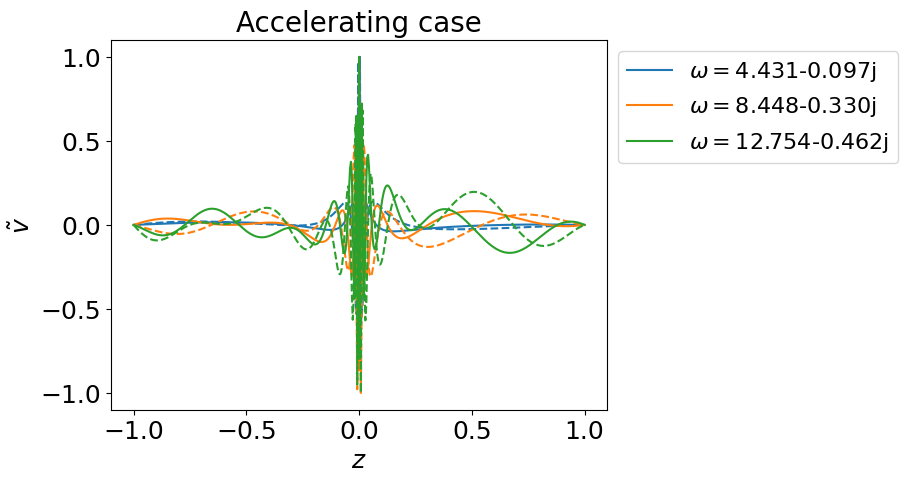
\includegraphics[width=0.95\textwidth]{figures/results-bad-accelerating-v.png}
  \end{center}
  \caption{Dirichlet boundary conditions are set at the two ends, all eigenfunctions are squeezed to the singular point.}
  \label{fig:bad-accelerating-v}
\end{figure}


After some investigation, we realized that there is a regular singular point at $z=0$. It is easy to see that from Eq.(\ref{eq:polynomial-eigenvalue-problem}) since the second order derivative term vanishes at $z=0$ due to the fact that $1-v_0^2=0$ at the sonic point.

\subsection{Singularity and Black hole}
Interesting enough, the acoustic perturbations of the gas fluid flow in the de Laval nozzle are proved to coincide with the quasi-normal modes of black holes solutions deformed by the 5D Weyl fluid. \cite{da_rocha_black_2017, furuhashi_simulation_2006} 

A quasi-1D fluid flow is ruled by the Euler-Lagrange equations and the continuity relation in fluid mechanics, given by
\begin{align} \label{eq:euler-lagrange}
  \pdv{t}(\rho A) + \pdv{x}(\rho A v) &= 0 \\
  \pdv{t}(\rho A v) + \pdv{x}[(\rho v^2 + p)A] &= 0 \\
  \pdv{t}\left(\frac{\rho v^2}{2} - \frac{p}{1-\gamma}A\right) +
  \pdv{x}\left[ \left(\frac{\rho v^2}{2} - \frac{\gamma}{1-\gamma}A\right)Av \right] &= 0
\end{align}

In \cite{da_rocha_black_2017, furuhashi_simulation_2006}, the so-called tortoise coordinate is introduced,
\[ x^* = c_{s0}\int [c_s(x)(1-M(x)^2)]^{-1} dx \]
where $c_{s0}$ denotes the stagnation speed of sound, $c_s = \dv*{p}{\rho}$ is the local speed of sound and $M(x)= v(x)/c_s(x)$ is the Mach number. Using the tortoise coordinate, the singularity is removed.

However, there are a few drawbacks in this method.
\begin{itemize}
  \item This method is complicated, we need to derive the Eq.(\ref{eq:polynomial-eigenvalue-problem}) in the new coordinate system.
  \item The new coordinate system pushes the singularity to infinity. However, we still need to cross the singularity in order to get the eigenvalues if we are using spectral method. 
\end{itemize}


\section{Boundary Condition at a Singular Point}
Some investigation leads us to a better method. To understand the logic flow, we need to realize that the singularity acts as an boundary condition for the problem. That means, we have no freedom to choose the boundary condition on the right once we fixed values of $\tilde{v}$ on the left boundary and at the singularity. We will illustrate this by expanding the solution at the singularity.

If we Taylor expand terms near the singularity, and only keep the first order term for the second order derivative term, Eq.(\ref{eq:polynomial-eigenvalue-problem}) becomes
\[ - 2v_0'(0)z\pdv[2]{\tilde{v}}{z}
+ (2i\omega - 4v_0'(0))\pdv{\tilde{v}}{z} 
+ (\omega^2 + 2i\omega v_0'(0) - 2v_0''(0))\tilde{v}
= 0 \]

Use Frobenius method, assuming $\tilde{v} = \sum_{n\geq 0}c_nz^{n+r}$, we get two different roots, $r=0$ and $r=1-a$. They correspond to finite solution and diverging solution near the singularity, respectively. The coefficients of the power series are given by 
where 
\begin{align*}    
  c_n &= \frac{(-1)^n b^n c_0}{\prod_{k=0}^{n-1} (n+r-k)(n+r-1+a-k)} \\
      &= (-1)^n b^n c_0 \frac{\Gamma(r+1)\Gamma(r+a)}{\Gamma(n+r+1)\Gamma(n+r+a)}
\end{align*}
where
\[ a = \frac{2i\omega - 4v_0'(0)}{-2v_0'(0)}; \quad 
  b = \frac{\omega^2 + 2i\omega v_0'(0) - 2v_0''(0)}{-2v_0'(0)}
\]

Worth to mention that the diverging solution goes like 
\[ 
\tilde{v}(z) \sim z^{1-a} = z^{-1-\omega_i/v_0'(0)}z^{i\omega_r/v_0'(0)}  \]
where $\omega = \omega_r + i\omega_i$. Meaning that the solution will be divergent iff $\omega_i > -v'(0)$.

This indicates that the regular solution that crosses the singularity smoothly are determined by two parameters only, $c_0$ and $\omega$. Once we choose $c_0$, the perturbation at the singularity, there is only one degree of freedom left, $\omega$. It seems reasonable to set the perturbation to 0 on the left boundary since it is the entrance of the magnetic nozzle. Now there is no more freedom to choose the boundary condition on the exit of the nozzle. 

\section{Shooting Method}

Shooting method can be used to solve eigenvalue problem with specified boundary values,
\begin{equation} \label{eq:boundary-eigenvalue-problem}
g(\tilde{v}(z);\omega) = 0,
\quad
z_l \leq z \leq z_r,
\quad
\tilde{v}(z_l) = \tilde{v}_l, \tilde{v}(z_r) = \tilde{v}_r
\end{equation}
where $\omega$ is the eigenvalue to be solved.

Suppose a eigenvalue problem can be formulated as
\[ \dv{z}\mathbf{u} = \mathbf{f}(\mathbf{u},z;\omega),
\quad
z_l<z<z_r,
\quad
\mathbf{u}(z_l) = \mathbf{u}_l
\]
where $\mathbf{u}\in\mathbb{R}^2$. Fixed an $\omega$, we can approximate $\mathbf{u}(z_r)$ by applying algorithms such as Runge-Kutta or Leap-frog.

Define $F$ by $F(\mathbf{u}_l;\omega)=\tilde{v}(z_r;\omega)$. This function $F$ takes in the initial value $\mathbf{u}_l$ and a fixed $\omega$, and outputs the "landing point" $\tilde{v}(z_r;\omega)$. If $\omega$ is an eigenvalue of Eq.(\ref{eq:boundary-eigenvalue-problem}), then $\tilde{v}(z_r;\omega) = \tilde{v}_r$. Now we can find eigenvalues to Eq.(\ref{eq:boundary-eigenvalue-problem}) by solving the roots to the scalar equation
\[h(\omega) = F(\mathbf{u}_l;\omega) - \tilde{v}_r\]

Having this higher view of shooting method in mind, we first transform Eq.(\ref{eq:polynomial-eigenvalue-problem}) to a IVP,
\begin{align*}
v' &= u\\
u' &= \frac{-1}{1-v_0^2}\left[
    \omega^2v + 2i\omega(v_0+v_0'v) - \left(3v_0 - \frac{1}{v_0}\right)v_0'u - \left(1-\frac{1}{v_0}^2\right)(v_0')^2v - \left(v_0+\frac{1}{v_0}v_0'' v\right)
\right]
\end{align*}
Since the singularity acts as a boundary condition, we can find the eigenvalues using the so-called shooting method. Starting from the singularity, we "shoot" the solution to the left using the technique for IVP (initial value problem). By matching the end point value to the left boundary condition, we can determine the eigenvalues. 

In order to get initially value for cases with transonic velocity profiles, we need the derivatives of $\tilde{v}$ at $z=0$. Since we already have the power series expansion of $\tilde{v}$ near singularity. Thus, we can obtain the initial conditions from the coefficients,
\begin{align*}
  v'(0) &= c_1 \\
  u'(0) &= v''(0) = 2c_2
\end{align*}

\subsection{Result}
By employing the shooting method, we are able to get eigenfunctions that crosses the singular point smoothly, see Fig.\ref{fig:good-accelerating-v}. We have no freedom to choose boundary condition on the right, the left boundary and the singular point determine the flow entirely.

\begin{figure}[htbp]
  \begin{center}
    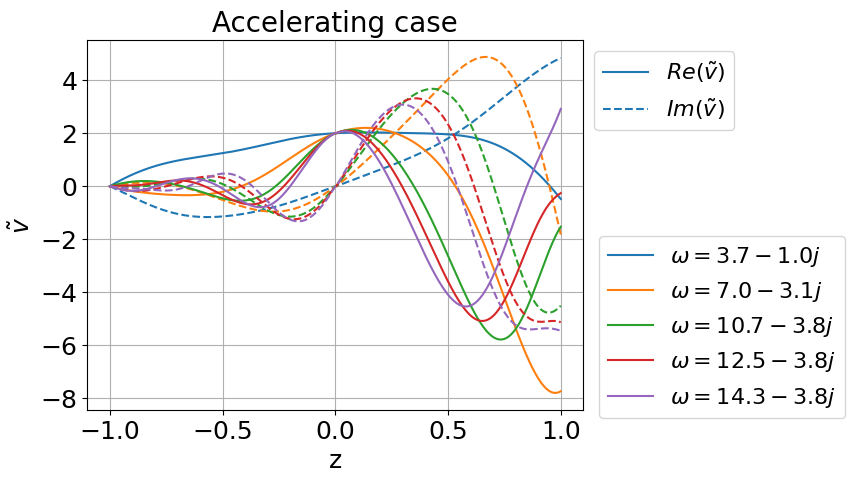
\includegraphics[width=0.7\textwidth]{figures/results-accelerating-v.png}
  \end{center}
  \caption{The solutions crosses the singular point smoothly. All modes are stable.}
  \label{fig:good-accelerating-v}
\end{figure}


